\documentclass{beamer}
\usepackage{verbatim} % For using /begin{comment}; /end{comment}
%--------------------------------------------------------------%
\usepackage{graphicx}
\definecolor{mine}{RGB}{155,155,155}
\definecolor{oj}{rgb}{1.0,0.65,0.0}
\definecolor{cblue}{rgb}{0.39, 0.58, 0.93}
\definecolor{turq}{rgb}{0.0, 0.81, 0.82}

\setbeamercolor{normal text}{bg=black, fg=white}
\setbeamercolor{title}{fg=turq}
\setbeamercolor{frametitle}{fg=oj}
\setbeamercolor{block title}{fg=green}
\setbeamercolor{itemize item}{fg=mine} % all frames will have red bullets
\setbeamercolor{enumerate item}{fg=mine} % all frames will have red bullets

\usefonttheme{serif}
\setbeamerfont{frametitle}{series=\bfseries} % Frame titles should be bold

\title{Basic Principles of Solar Acoustic Holography}
\subtitle{ASTR 500}
\date{11 March 2016}
\author{Laurel Farris}

\begin{document}

\begin{frame}
    \titlepage
\end{frame}

\begin{frame}{Outline}
    \begin{enumerate}
        \item Introduction
        \item Basic Principles of Computational Seismic Holography
        \item The Computational Task
        \item Subjacent Vantage Holography
        \item An Example
        \item Acoustic Modelling Based on Holographic Images
        \item Phase-Sensitive Holography
        \item Green's Functions
        \item Summary
    \end{enumerate}
\end{frame}

\begin{frame}
    ``Seismic holography'' was applied to helioseismic data from SOHO.
    New solar acoustic phenomena:
    \begin{itemize}
        \item `acoustic moats' surrounding sunspots
        \item `acoustic condensations' 10-20 Mm beneath active regions
        \item `acoustic glories' surrounding complex active regions
        \item first helioseismic images of a flare
    \end{itemize}
\end{frame}

\begin{frame}{Figure 1}
    \begin{figure}
        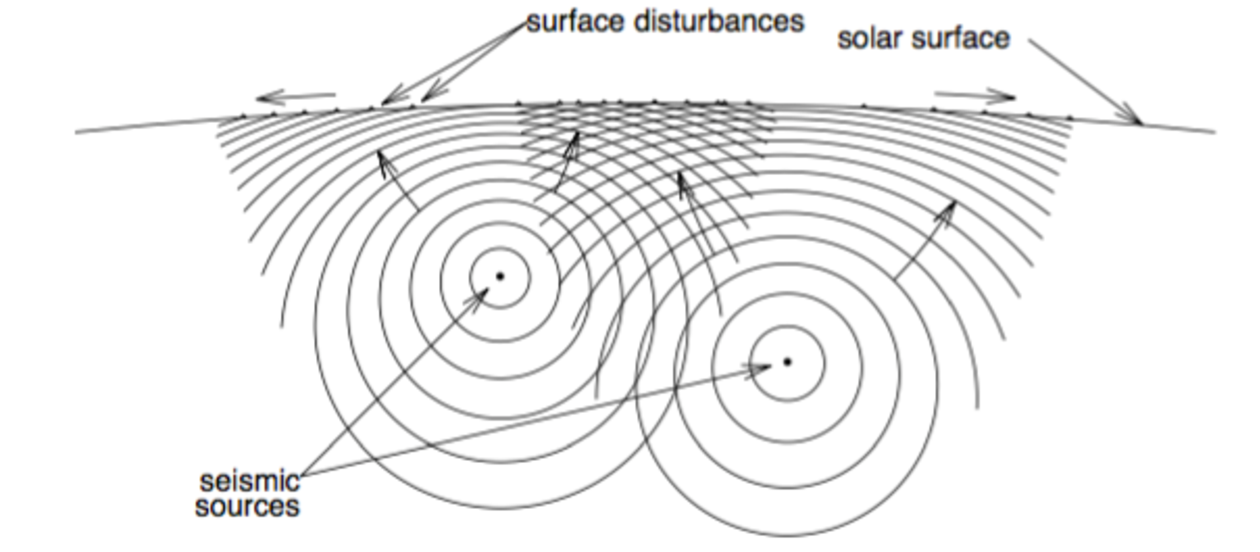
\includegraphics[width=0.8\textwidth]{fig_1.pdf}
        \caption{captiontext}
    \end{figure}
\end{frame}

\begin{frame}{Figure 2}
    \begin{figure}
        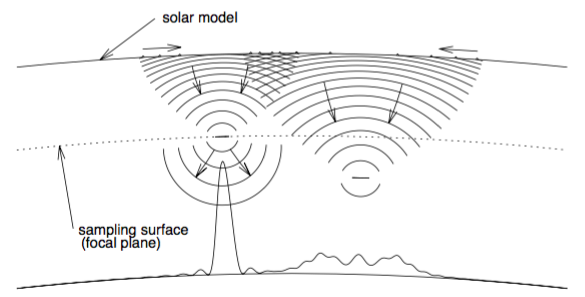
\includegraphics[width=0.8\textwidth]{fig_2.png}
        \caption{captiontext}
       % \label{figurelabel}
    \end{figure}
\end{frame}

\begin{frame}{Figure 3}
    \begin{figure}
        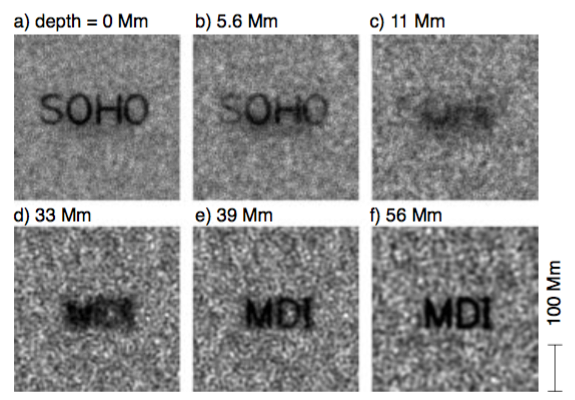
\includegraphics[width=0.8\textwidth]{fig_3.png}
        \caption{captiontext}
       % \label{figurelabel}
    \end{figure}
\end{frame}

\begin{frame}{Figure 4}
    \begin{figure}
        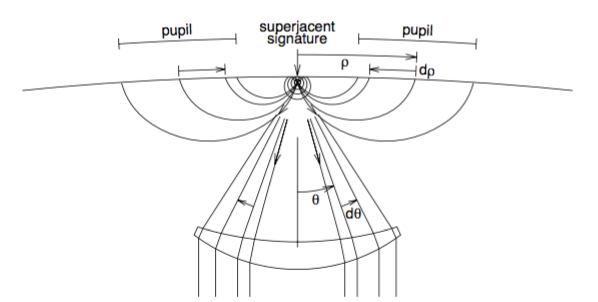
\includegraphics[width=0.8\textwidth]{fig_4.png}
        \caption{captiontext}
       % \label{figurelabel}
    \end{figure}
\end{frame}

\begin{frame}{Figure 5}
    \begin{figure}
        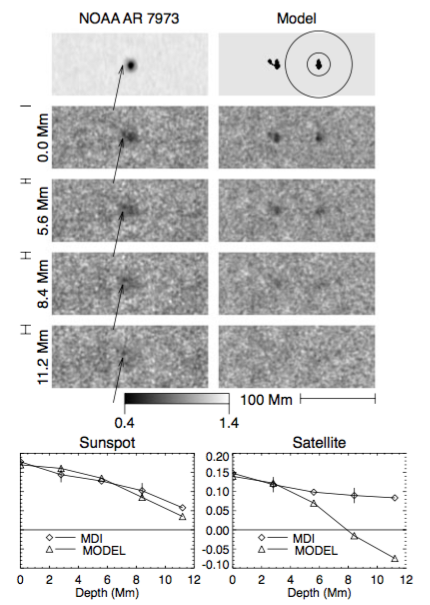
\includegraphics[width=0.8\textwidth]{fig_5.png}
        \caption{captiontext}
       % \label{figurelabel}
    \end{figure}
\end{frame}

\begin{frame}{Figure 6}
    \begin{figure}
        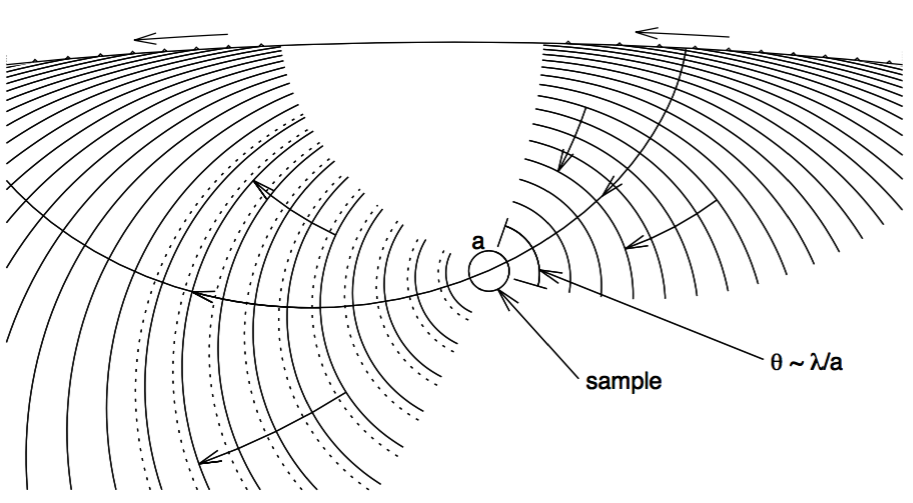
\includegraphics[width=0.8\textwidth]{fig_6.png}
        \caption{captiontext}
       % \label{figurelabel}
    \end{figure}
\end{frame}

\begin{frame}{Figure 7}
    \begin{figure}
        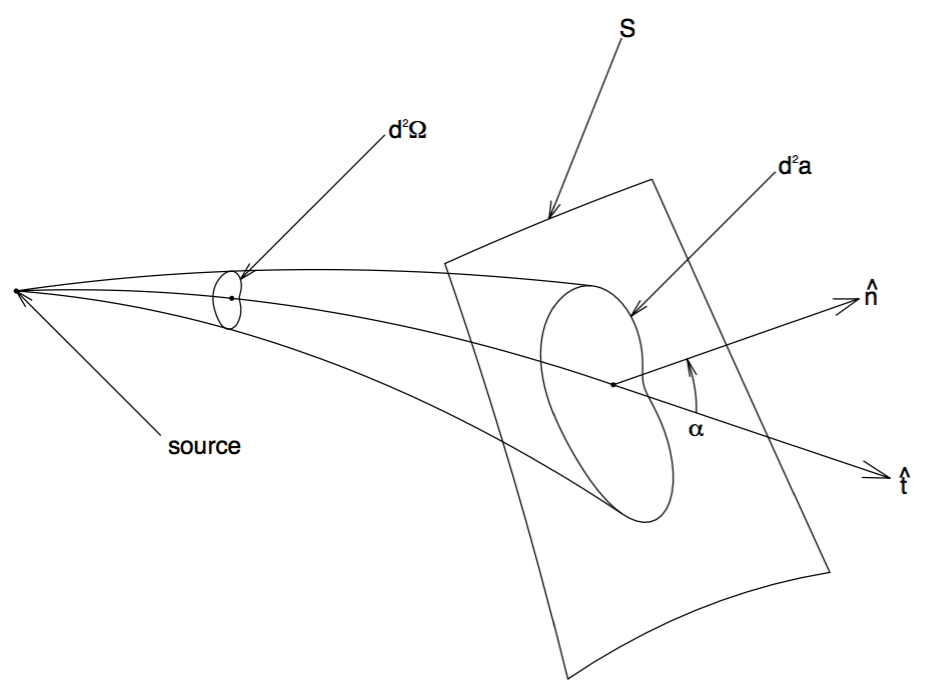
\includegraphics[width=0.8\textwidth]{fig_7.png}
        \caption{captiontext}
       % \label{figurelabel}
    \end{figure}
\end{frame}

\begin{frame}{Figure 8}
    \begin{figure}
        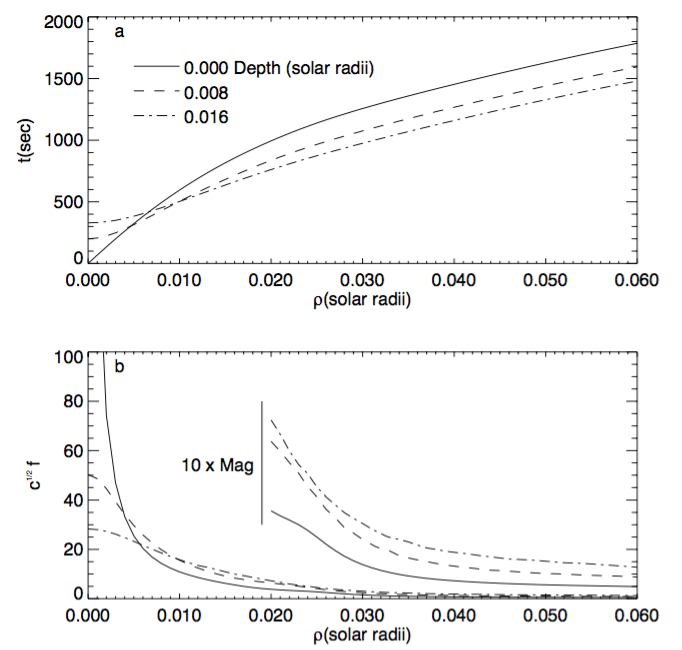
\includegraphics[width=0.8\textwidth]{fig_8.png}
        \caption{captiontext}
       % \label{figurelabel}
    \end{figure}
\end{frame}

\begin{frame}{Figure 9}
    \begin{figure}
        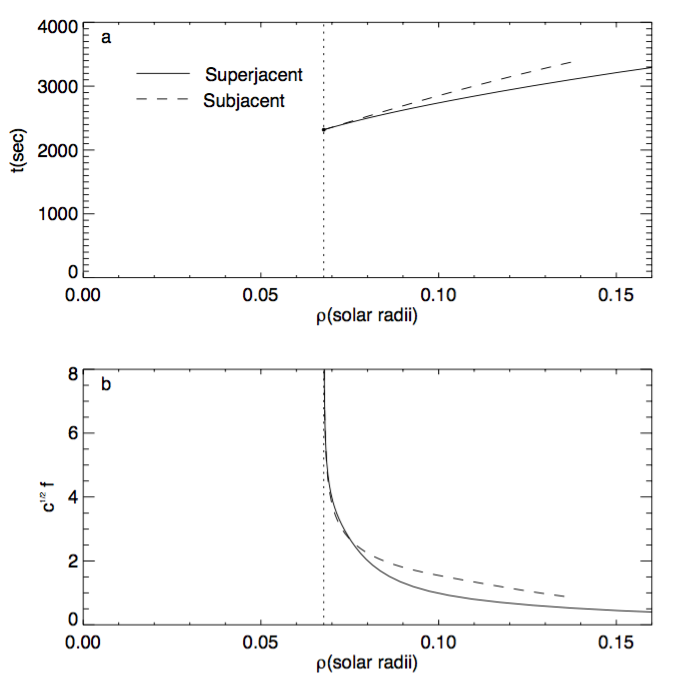
\includegraphics[width=0.8\textwidth]{fig_9.png}
        \caption{captiontext}
       % \label{figurelabel}
    \end{figure}
\end{frame}

\begin{frame}{Figure 10}
    \begin{figure}
        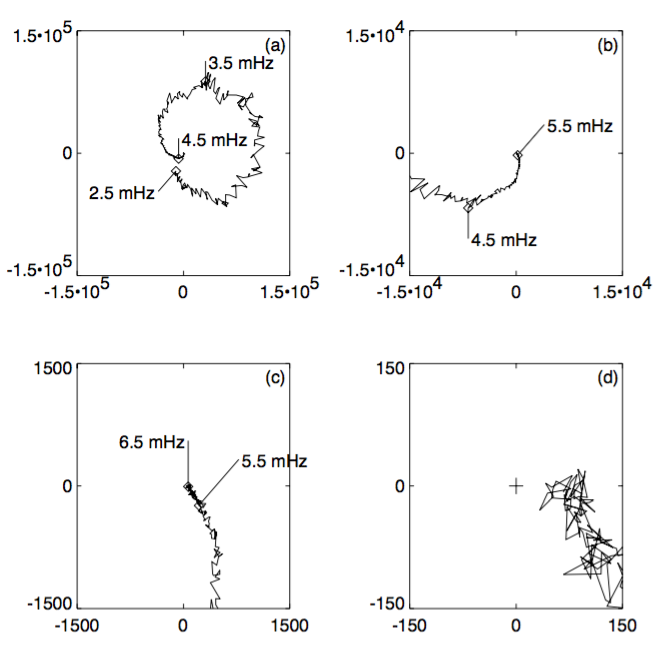
\includegraphics[width=0.8\textwidth]{fig_10.png}
        \caption{captiontext}
       % \label{figurelabel}
    \end{figure}
\end{frame}

\begin{frame}{Figure 11}
    \begin{figure}
        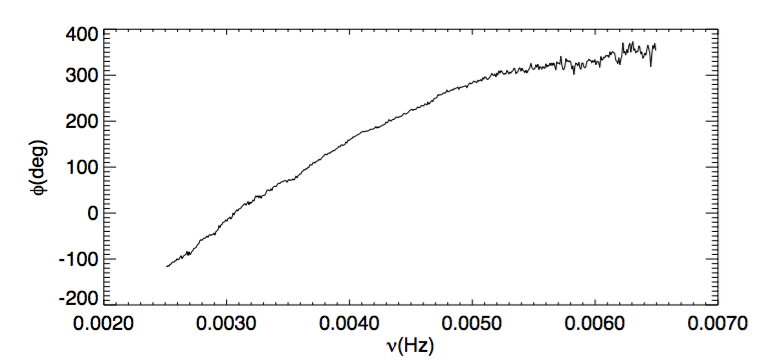
\includegraphics[width=0.8\textwidth]{fig_11.png}
        \caption{captiontext}
       % \label{figurelabel}
    \end{figure}
\end{frame}
%--------------------------------------------------------------%

\end{document}
